\section{Results}
\label{sec:results}
In \Cref{sec:ablations} we first focus on understanding the impact of
the main components of our training setup on performance as measured
by recall@10 and triplet accuracy. Afterwards in
\Cref{sec:minimal-pairs} we switch our attention to the targeted
evaluation via minimal pairs.
\todo{GC: We really should have at least 3 runs of each configuration with a different random seed.}


\subsection{Ablations}
\label{sec:ablations}
For completeness, we report results on both the dialog and narration
data. However, it should be kept in mind that in the case of the
narration data the scores are not confounded by speaker-based clues
and thus the scores on narration are those that indicate to what extent to
model learns aspects of utterance meaning.

\todo{GC: Generate and insert results on test data}
\subsubsection{Pre-training and Fine-tuning}
Results on different pre-training configurations are shown in
\Cref{fig:pretraining}.
\begin{figure}[htb]
	\centering
	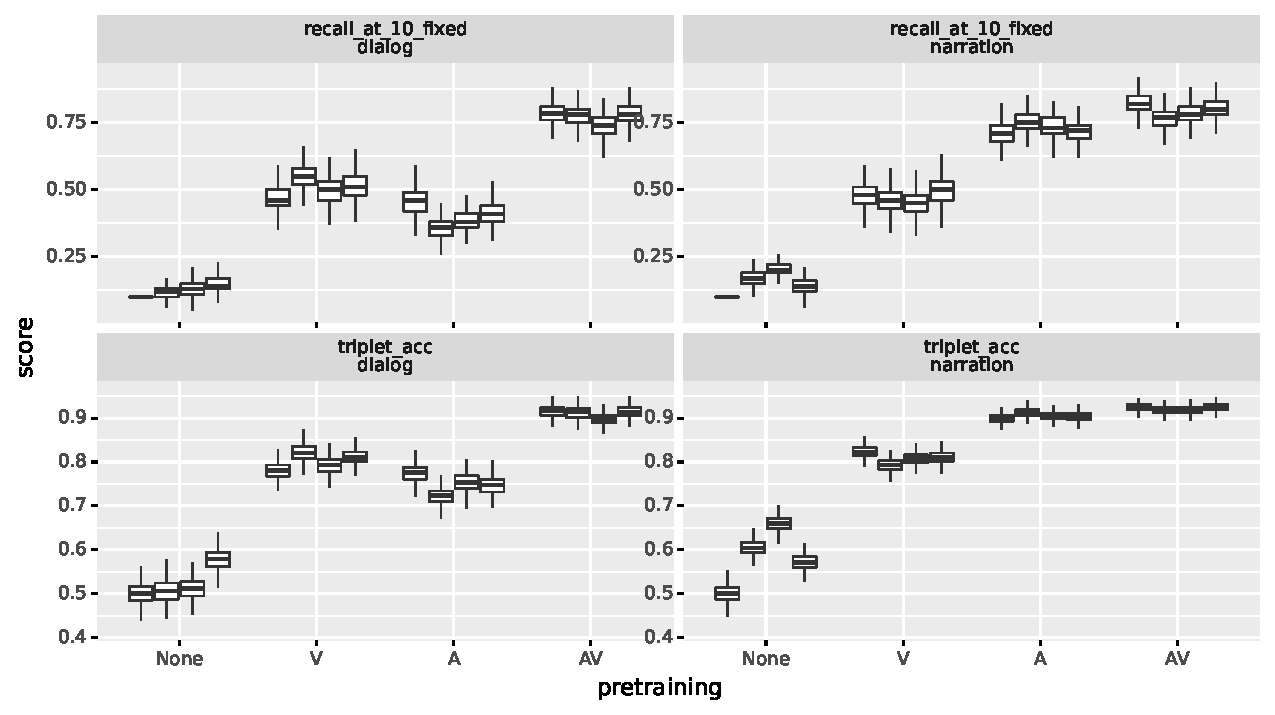
\includegraphics[width=\columnwidth]{results/ablations/pretraining.pdf}
	\caption{Effect of pre-training on performance on the dialog
          and narration validation data. The top row shows recall@10;
          the bottom row triplet accuracy.}
	\label{fig:pretraining}
      \end{figure}

The best overall performance on both the dialog and the narration data is 
achieved with a model where both the video and audio encoder are pre-trained 
before being fine-tuned on our data. The model with no pre-training in
either modality failed to converge and thus performs at random.


On narration data, for both metrics, we see a clear ranking of
configurations from best to worst: (AV) audio and video pre-training,
(A) audio pre-training, (V) video pre-training and (None) no
trainining. Meanwhile for dialog data, the performance between A and V
is comparable.

%A model that is trained on scratch using only our data performs still 
%substantially above chance on all metrics ($0.1$ for recall@10 and $0.5$ for 
%triplet accuracy). \todo{MN: Do we maybe want to add the chance (random 
%guessing) baselines into the plots? }

To further understand and disentangle the effects of audio pre-training and 
fine-tuning, we train a model with frozen parameters of the 
\textsc{wav2vec} module. The effect of this condition is show in \Cref{fig:freeze_wav2vec}.
\begin{figure}[htb]
  \centering
  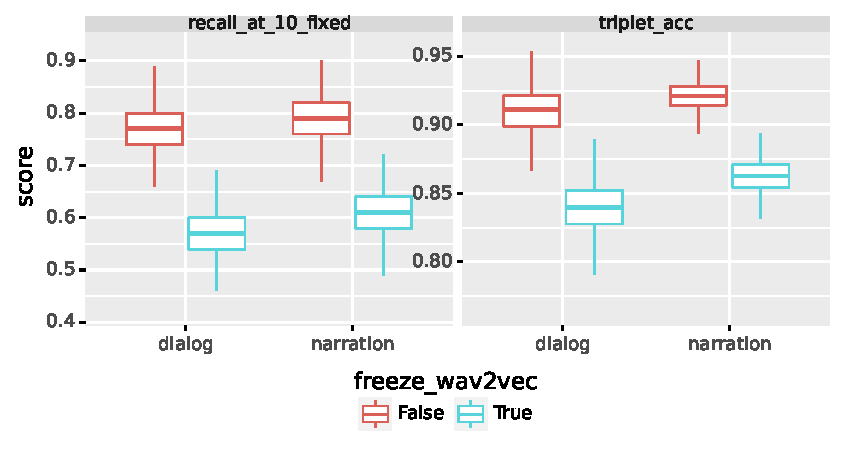
\includegraphics[width=\columnwidth]{results/ablations/freeze_wav2vec.pdf}
  \caption{Effect of freezing the parameters of the \textsc{wav2vec}
    module on model performance, on the dialog and narration
    validation data. The top row shows recall@10; the bottom row
    triplet accuracy.}
  \label{fig:freeze_wav2vec}
\end{figure}
We find without fine-tuning of the \textsc{wav2vec} module, performance decreases substantially 
on both metrics. In other words, best performance is only achieved with pre-trained and 
fine-tuned models.


\subsubsection{Jitter}
Next, we evaluate a model that has been trained with varying video and audio 
lengths (\textsc{jitter}). For fair comparison, we report recall@10 for both 
\textsc{fixed} and \textsc{jitter} validation configurations.
As seen in \Cref{fig:jitter}, the effect of \textsc{jitter} is only
minor and that performance is comparable. \todo{GC: Insert reference
  to results with jitter for minimal pair scenario.}
\begin{figure}[htb]
	\centering
	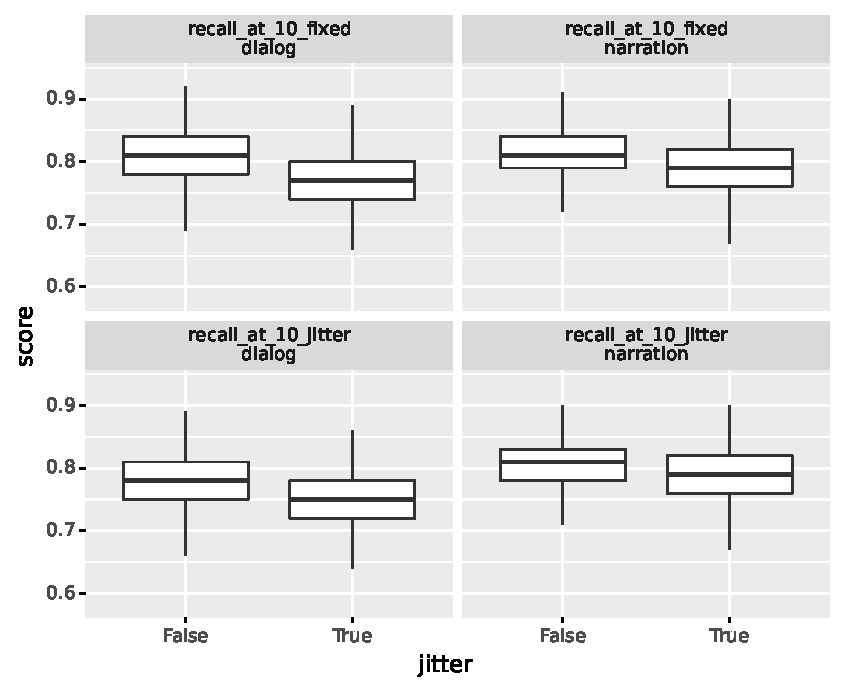
\includegraphics[width=\columnwidth]{results/ablations/jitter.pdf}
	\caption{Effect of jitter on model performance, on the dialog
          and narration validation data. The top row shows recall@10;
          the bottom row triplet accuracy.}
	\label{fig:jitter}
\end{figure}



\subsubsection{Temporal Information}
Finally, we explore the role of the temporal nature of the visual
modality.  \Cref{fig:static} compares the model with the regular video
encoder with one using the \textsc{static} baseline encoder. Across
all metrics, we observe substantial performance drops for the
\textsc{static} model, which has access to the same video frames, but
does not have access to their temporal ordering. \todo{GC: Note that a
  confounding factor here is that the static encoder is pre-trained on
  ImageNet rather than Kinetics. Maybe we should instead compare
  models without video pre-training.}

\begin{figure}[htb]
  \centering
  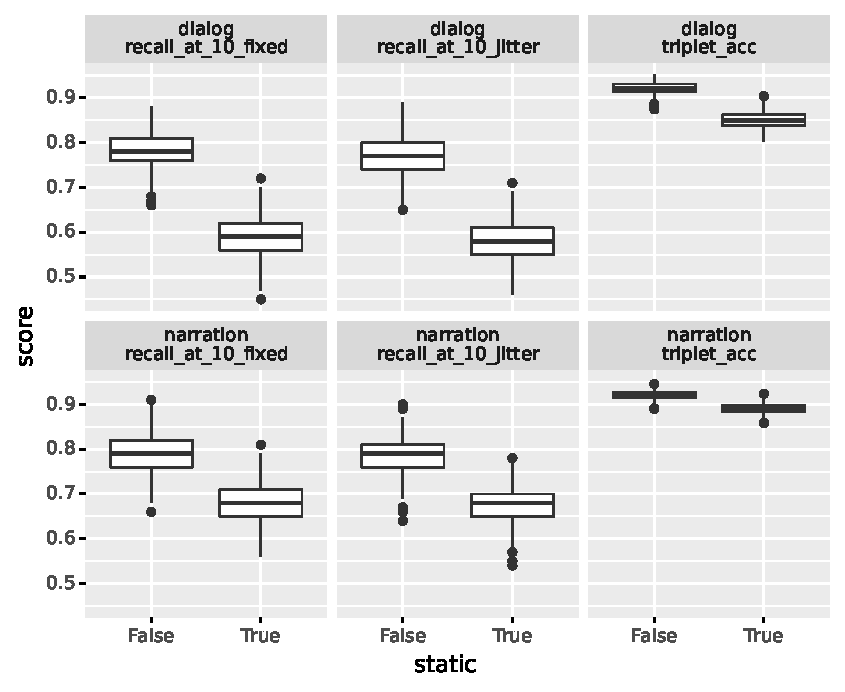
\includegraphics[width=\columnwidth]{results/ablations/static.pdf}
  \caption{Effect of temporal information on model performance, on the dialog
          and narration validation data. The top row shows recall@10;
          the bottom row triplet accuracy.}
  \label{fig:static}
\end{figure}


\subsection{Minimal Pairs}
\label{sec:minimal-pairs}


\Cref{tab:minimal_pair_results} presents results for the minimal pair 
evaluation. We find that a models that are 
pre-trained and fine-tuned with \textsc{jitter} perform best. Generally, there 
is not much difference in the scores for verbs and nouns, with the exception of 
models trained on \textsc{static} data. Here the performance for verbs is 
worse, confirming that temporal information is more important for the semantics 
of verbs.
\todo{Keep table? Add more rows?}
\begin{table}[ht]
	\centering
	\begin{tabular}{lllll}
		\toprule
		& & & \multicolumn{2}{c}{Accuracy} \\
		Finetune & Jitter & Static & Nouns & Verbs \\
		\midrule
		\checkmark & \checkmark &  & 0.81 & 0.80 \\
		\checkmark &  &  & 0.73 & 0.73  \\
		 & \checkmark &  & 0.71 & 0.70 \\
		\checkmark & \checkmark &  \checkmark & 0.79 & 0.76 \\
		\bottomrule
	\end{tabular}
	\caption{Minimal pair accuracies for different model configurations.}
	\label{tab:minimal_pair_results}
\end{table}
%We report results for our evaluation with minimal pairs for the best 
%performing 
%models as identified in the previous section (audio and video pre-training + 
%\textsc{jitter}).

\Cref{fig:accuracy_targeted_triplets_nouns} and
\ref{fig:accuracy_targeted_triplets_verbs} show per-word
accuracy for nouns and verbs for the best performing model.
We perform bootstrapping (n\_resampling = 100) to estimate mean and standard 
deviation for each accuracy score.


\begin{figure*}[htb]
  \centering
  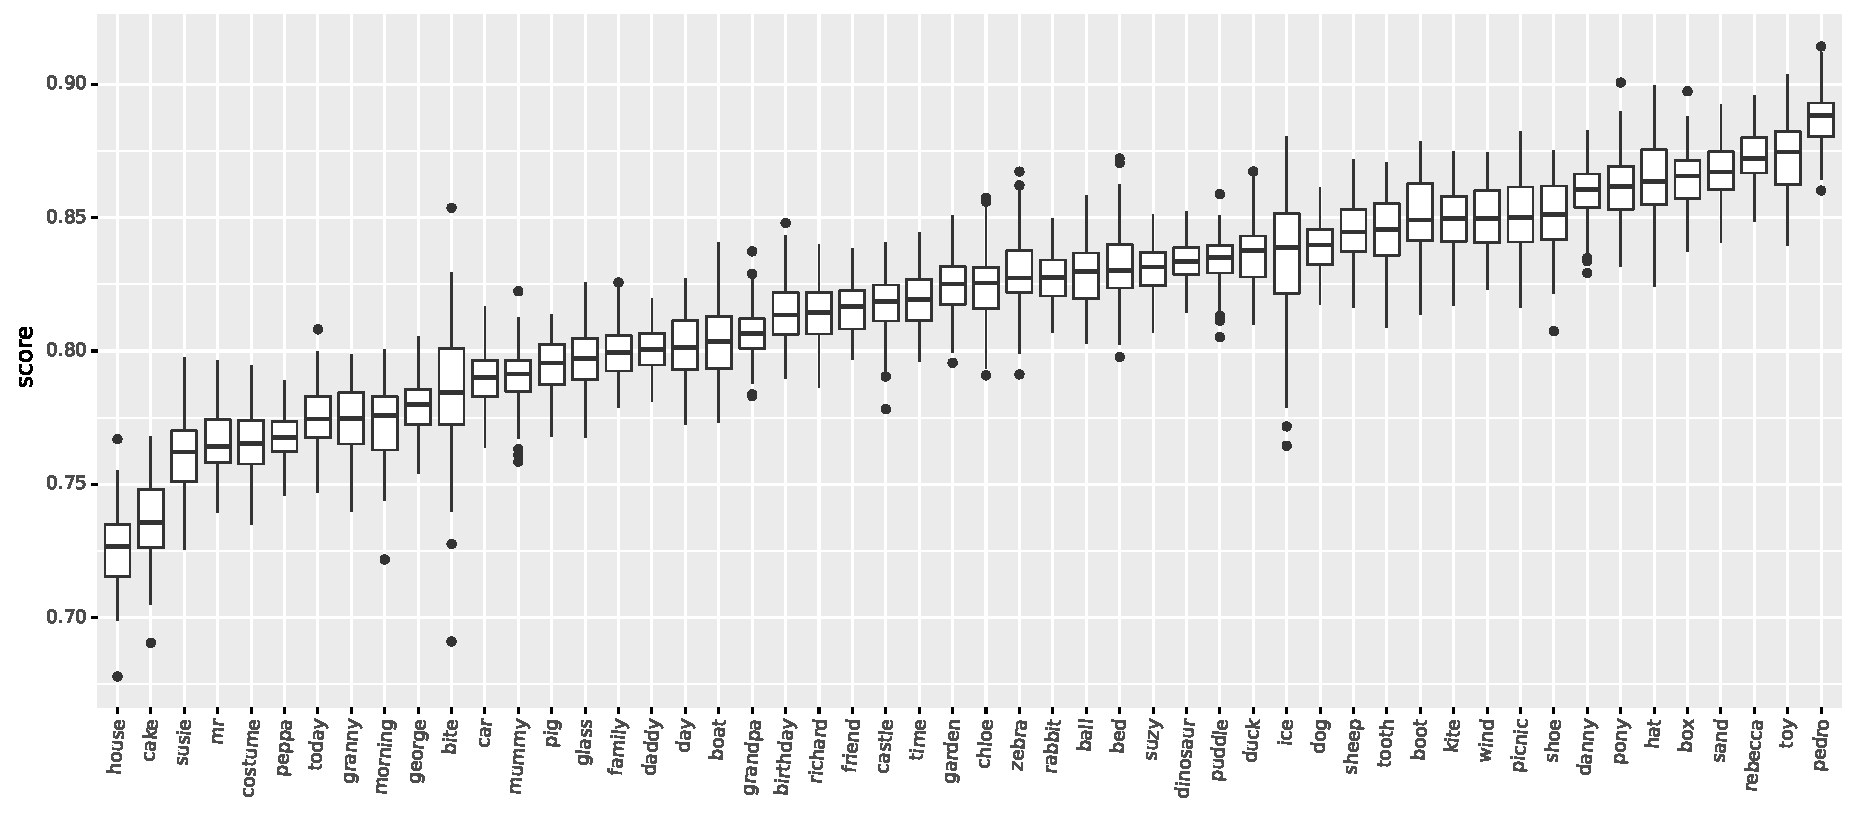
\includegraphics[width=\textwidth]{results/targeted_triplets/results_per_word_version_335_NOUN.pdf}
  \caption{Per-word accuracies on the minimal pairs evaluation data for nouns.}
  \label{fig:accuracy_targeted_triplets_nouns}
\end{figure*}

\begin{figure}[htb]
  \centering
  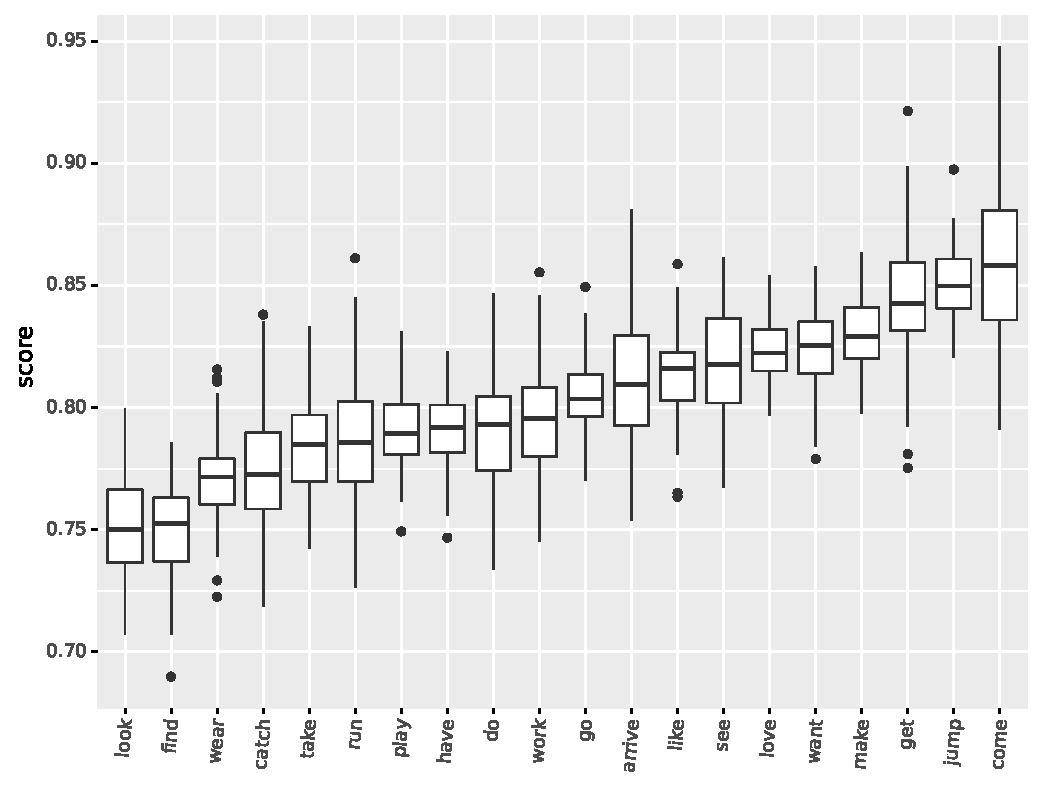
\includegraphics[width=\linewidth]{results/targeted_triplets/results_per_word_version_335_VERB.pdf}
  \caption{Per-word accuracies on the minimal pairs evaluation data
    for verbs.}
  \label{fig:accuracy_targeted_triplets_verbs}
\end{figure}

We observe substantial variance in the accuracy scores, suggesting that the 
difficulty to learn certain words varies. For example, the 
scores for ``house'' and ``cake'' are very low. This could be because these 
concepts are not easy to ground, as they do not often refer to a similar visual 
entity. When looking at our evaluation examples, we find that indeed the word 
``house'' is used in varying visual contexts (house entrance, view of the whole 
house, inside the house, rabbit's house) and in displaced speech (talking about 
going to somebody's house). Regarding ``cake'', it refers to either a whole 
cake, a slice, dough, or crumbs.

On the other end, the words ``Pedro'' and ``Rebecca'' are learned very well: 
They refer to ``Pedro pony'' and ``Rebecca rabbit'', easily visually 
distinguishable from other characters which are mainly pigs. Additionally, it 
is usually present and central to the video when mentioned.

Further investigations with larger datasets are necessary to reveal the 
underlying reasons for difficulty, and relating them to predictors of age of 
acquisition in the child language acquisition literature 
\cite{roy2015predicting,frank2021variability}. 


